%% LaTeX Beamer presentation template (requires beamer package)
%% see http://latex-beamer.sourceforge.net/
%% idea contributed by H. Turgut Uyar
%% template based on a template by Till Tantau
%% this template is still evolving - it might differ in future releases!

\documentclass{beamer}
\usetheme{Freiburg}
%\usepackage{german}
%\usepackage[utf8]{inputenc}
\usepackage[ngerman]{babel}
%\usepackage[pdftex]{graphicx}
%\usepackage{epstopdf}
%\usepackage{subfig}
%\usepackage[cmex10]{amsmath}
%\usepackage{dsfont}
%\usepackage{IEEEtrantools}
%\usepackage[nocites]{refcheck}
%\usepackage[colorlinks=true,linkcolor=black]{hyperref} 

% Anmerkungen
%\usepackage{pgfshade}
\usepackage{pgfpages}
%\setbeameroption{show notes on second screen}

% dynamisches Highlithing
\def\hilite<#1>{\temporal<#1>{\color{gray}}{\color{blue!20!red!60!black}}{\color{black}}}
\def\hilitealert<#1>{\temporal<#1>{\color{gray}}{\color{red!60!black}}{\color{black}}}

%================================================================
%================================================================

\begin{document}

%================================================================
%================================================================

\title[Flexible Ortung]{Flexible Ortung von Schwarmelementen im Innenraum auf
Basis kosteng\"unstiger Kameras}
%\subtitle{Verteidigung der Bachelorarbeit}
\author{Angelos Drossos} 
\institute{\Large Technische Universit"at Berlin\\\large Fakult"at IV --
Elektrotechnik und Informatik\\Fachgebiet Kommunikations- und Betriebssysteme}
\date{\today}
\logo{
\includegraphics[scale=0.45]{logo_tub.png}}

%================================================================
%================================================================

\begin{frame}%[plain]
	\frametitle{Verteidigung der Bachelorarbeit}
	\titlepage
\end{frame}

\note[itemize]{
	\item Begr\"u"ssung: 
	\item Sehr geehrte Mitglieder der TU-Berlin 
	\item s. g. Damen \& Herren
	\item gerne pr\"asentiere ich Ihnen meine Bachlorarbeit
	\item zum Thema ``Flexible Ortung von Schwarmelmenten im Innenraum ..
	\item .. auf Basis kosteng\"unstiger kameras''
	\item Zun\"achst zu meiner Person: Ich bin Angelos Drossos.
	\item Ich beende mit diesem Vortrag meinen Bachelor in Technischer Informatik 
	\item und habe bereits meinen Master ``Angewandte Informationstechnologien'' 
	\item mit der Spezialisierung ``Intelligente Informations- und Kommunikationstechnologien''
	\item begonnen.
}

%================================================================
%================================================================

\section{Einf\"uhrung}

%----------------------------------------------------------------

\begin{frame}
	\frametitle{Einf\"uhrung}\framesubtitle{Schw\"arme in der Natur}
	
	\begin{columns}
		\begin{column}{0.5\textwidth}
			\begin{figure}
				\centering
				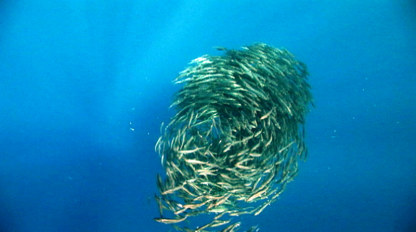
\includegraphics[width=\textwidth]{bilder/Schwarm_Fische2.jpg}
				\caption{Wie viele Fische befinden sich im Schwarm?}
			\end{figure}
		\end{column}
		\begin{column}{0.5\textwidth}
			\begin{figure}
				\centering
				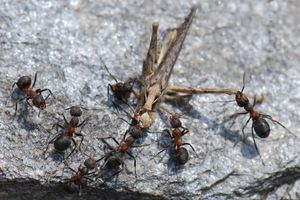
\includegraphics[width=\textwidth]{bilder/Ameisen_jagen_Wurm.jpg}
				\caption{Ameisen jagen gemeinsam eine Heuschrecke}
			\end{figure}
		\end{column}
	\end{columns}
	
\end{frame}

\note[itemize]{
	\item Die Idee eines Super-organismus mit Schwarmintelligenz faszinierte viele Forscher -- sowohl in der Biologie wie auch in der Robotik.
	\item Daher m\"ochte ich Ihnen die Vorbilder der Natur zeigen.
	\item Auf dem linken Bild:\\
			Ein Schwarm Fische, beispielsweise Meer\"aschen. Sie schwimmen in einer gro"ssen Gruppe.\\
			Ihre genaue Zahl ist schwer zu sch\"atzen und von weitem betrachtet wirken sie wie ein gro"sser Fisch.\\
			Und dies sind nur ein paar Vorteile..
	\item Ameisen bilden ebenfalls ``Schw\"arme'', auch wenn dies nicht gleich im rechten Bild erkennbar ist.\\
			Sie hinterlassen einen Duft, den andere Ameisen erkennen und diesem Folgen.
			Auf diese Weise zeigen sie anderen den Weg, hier zu einer Heuschrecke.
			Angriff Gegner, bla.. 
}

%================================================================

\subsection{Motivation}

%----------------------------------------------------------------

\begin{frame}
	\frametitle{Motivation}\framesubtitle{Schwarmintelligenz in der Natur}
	\note[item]{\notecurr<1> V\"ogel und Bienen - Schwarmtiere}
	\begin{columns}
		\begin{column}{0.30\textwidth}
			\begin{figure}
				\centering
				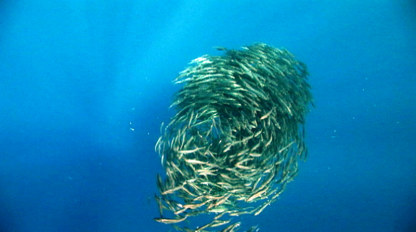
\includegraphics[width=\textwidth]{bilder/Schwarm_Fische2.jpg}
			\end{figure}
		\end{column}
		\begin{column}{0.224\textwidth}
			\begin{figure}
				\centering
				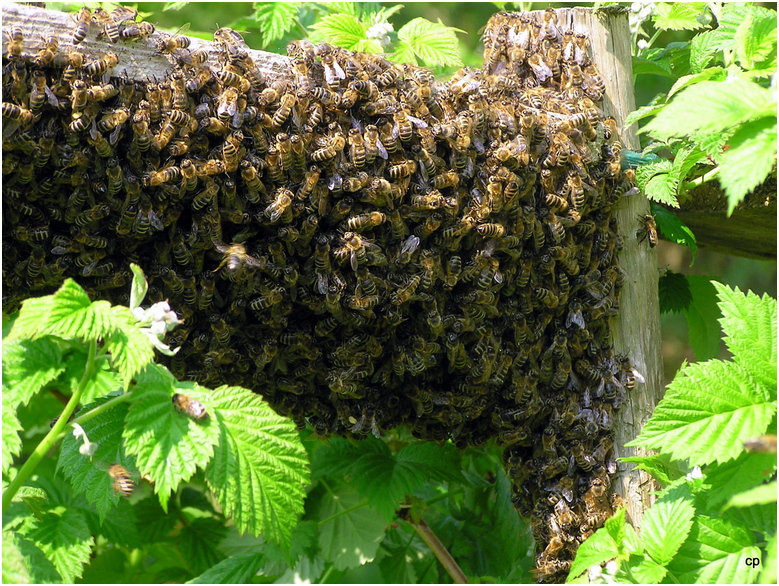
\includegraphics[width=\textwidth]{bilder/Schwarm_Bienen2.jpg}
			\end{figure}
		\end{column}
		\begin{column}{0.25\textwidth}
			\begin{figure}
				\centering
				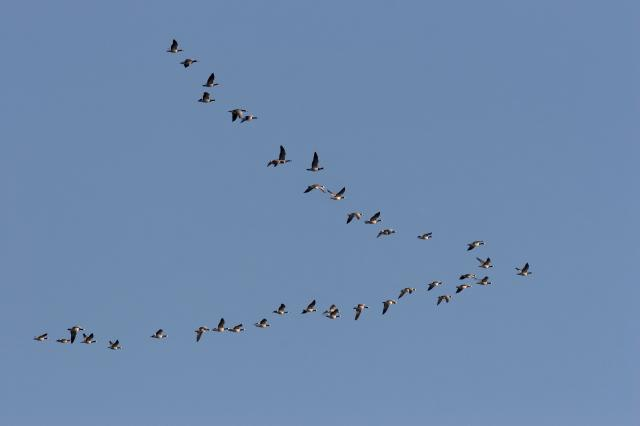
\includegraphics[width=\textwidth]{bilder/Schwarm_Voegel.jpg}
			\end{figure}
		\end{column}
		\begin{column}{0.25\textwidth}
			\begin{figure}
				\centering
				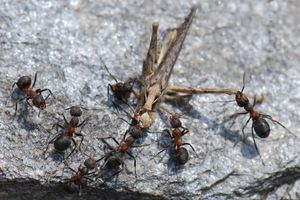
\includegraphics[width=\textwidth]{bilder/Ameisen_jagen_Wurm.jpg}
			\end{figure}
		\end{column}
	\end{columns}
	\note[item]{\notecurr<1> Beispiel - Fische:}
	\begin{exampleblock}<+->{Vorteile --- Am Beispiel der Fische}
		\begin{itemize}
		  \hilite<2> \item Schw\"achere ben\"otigen weniger Energie zum Fortbewegen\note[item]{\notecurr<2> Schw\"acherer im Mittelfeld - nutzen Str\"omungsfeld der vorderen - weniger Energie}
		  \hilite<3> \item St\"arkere bekommen mehr Futter\note[item]{\notecurr<3> zum ausgleich: vorderen/st\"arkeren schwimmer mehr futter}
		  \hilite<4> \item Schnelles Erkennen von Gefahren\note[item]{\notecurr<4> Ein fisch - Gefahr - Auseinanderschwimmen}
		  \hilite<5> \item Angreifer k\"onnen sich beim Angreifen verletzen\note[item]{\notecurr<5> dichte des schwarms kann angreifer verunsichert werden}
		  \hilite<5> \item Angreifer kann sich nicht auf ein Einzelnen konzentrieren\note[item]{\notecurr<5> durch blitzschnelles auseinanderschwimmen, keine konzentration auf einen einzelnen}
		\end{itemize}
	\end{exampleblock}
	\note[item]{\notecurr<5> Schwarmtiere \"uberblicken nicht die Gesamtsituation, doch sch\"atzen sie die Vorteile.}
	\note[item]{\notecurr<5> dadurch dass sie sich andere verlassen, entsteht eine Schwarmintelligenz, ein Super-Organismus}
\end{frame}

%----------------------------------------------------------------

\subsection{Ziel}

%----------------------------------------------------------------

\begin{frame} 
	\frametitle{Ziel}\framesubtitle{Schwarmintelligenz in der Robotik}
	
	\begin{columns}
		\begin{column}{0.30\textwidth}
			\begin{figure}
				\centering
				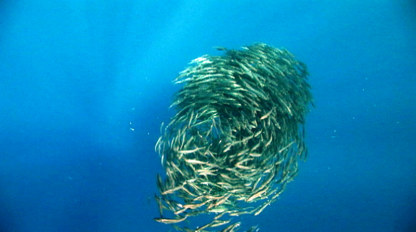
\includegraphics[width=\textwidth]{bilder/Schwarm_Fische2.jpg}
			\end{figure}
		\end{column}
		\begin{column}{0.224\textwidth}
			\begin{figure}
				\centering
				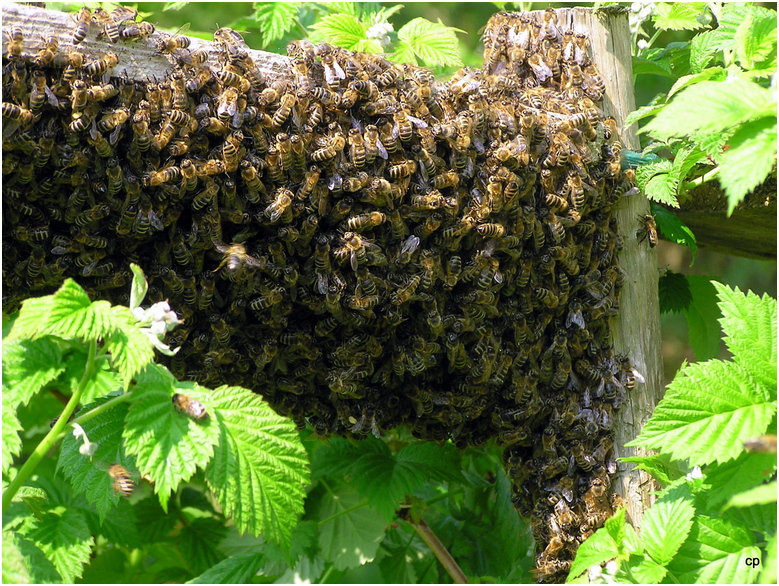
\includegraphics[width=\textwidth]{bilder/Schwarm_Bienen2.jpg}
			\end{figure}
		\end{column}
		\begin{column}{0.25\textwidth}
			\begin{figure}
				\centering
				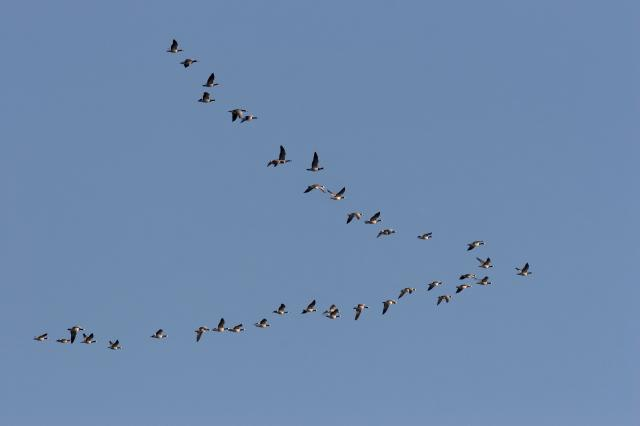
\includegraphics[width=\textwidth]{bilder/Schwarm_Voegel.jpg}
			\end{figure}
		\end{column}
		\begin{column}{0.25\textwidth}
			\begin{figure}
				\centering
				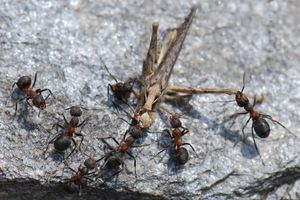
\includegraphics[width=\textwidth]{bilder/Ameisen_jagen_Wurm.jpg}
			\end{figure}
		\end{column}
	\end{columns}
	
	\note[item]{Typische Merkmale:}
	\note[item]{Kollektivverhalten}
	\note[item]{Strategie}
	\note[item]{Formationsbildung}
	\note[item]{Grunds\"atze -- Schwarmintelligenz}
	
	
	\begin{block}<+->{Schwarmintelligenz: Grunds\"atze}
		\begin{enumerate}
		  \hilite<1> \item Kollisionen sind zu vermeiden
		  \hilite<2> \item Der Durchsschnittsabstand zu den Nachbarn ist konstant zu halten
		  \hilite<3> \item Die eigene Richtung und Geschwindigkeit orientiert sich an der der unmittelbaren Nachbarn
		\end{enumerate}
	\end{block}
	
	\hilitealert<4> Allgemeines Ziel: Einhalten solcher Grunds\"atze
	
	\hilitealert<5> Konkretes Ziel: Bestimmung der Position der Schwarmelemente
	
\end{frame}

%================================================================
%================================================================

\section{Problemanalyse}

%----------------------------------------------------------------

\begin{frame}\frametitle{Inhaltsverzeichnis}\framesubtitle{Problemanalyse}
\tableofcontents[currentsection, hidesubsections]
\end{frame}

%----------------------------------------------------------------

\subsection{System}

%----------------------------------------------------------------

\begin{frame}
	\frametitle{System}\framesubtitle{Schwarmelemente}
	\begin{columns}
		\begin{column}{0.5\textwidth}
			\begin{figure}
				\centering
				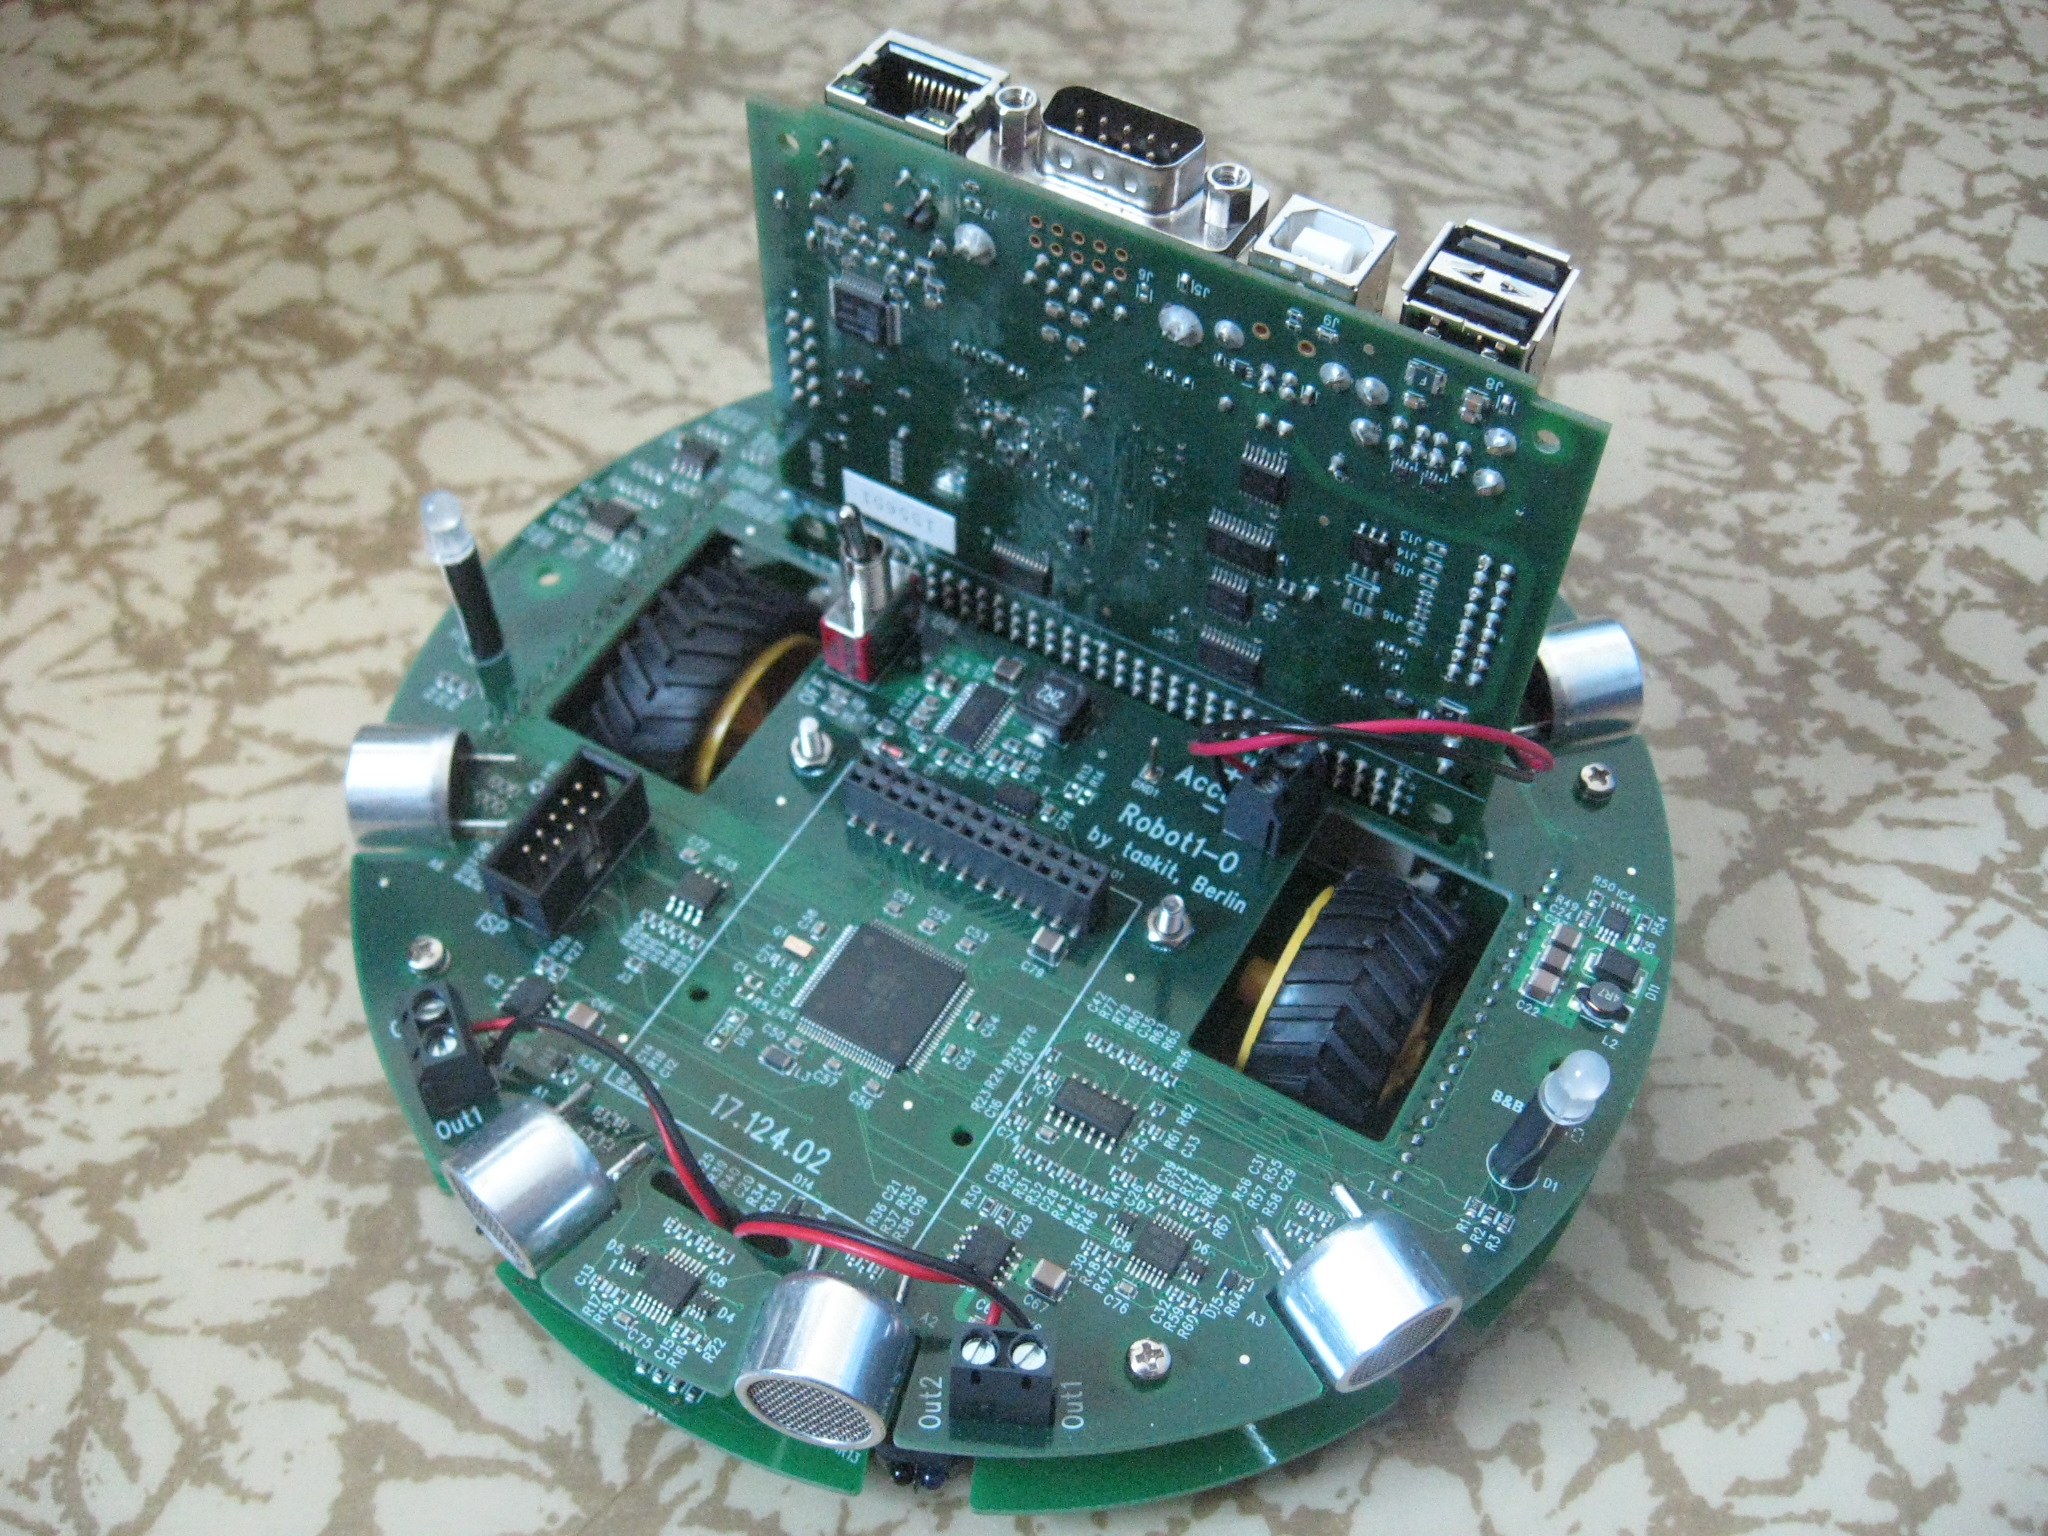
\includegraphics[width=\textwidth]{bilder/robo1.jpg}
				\caption{Schwarmelement von vorn}
			\end{figure}
		\end{column}
		\begin{column}{0.5\textwidth}
			\begin{figure}
				\centering
				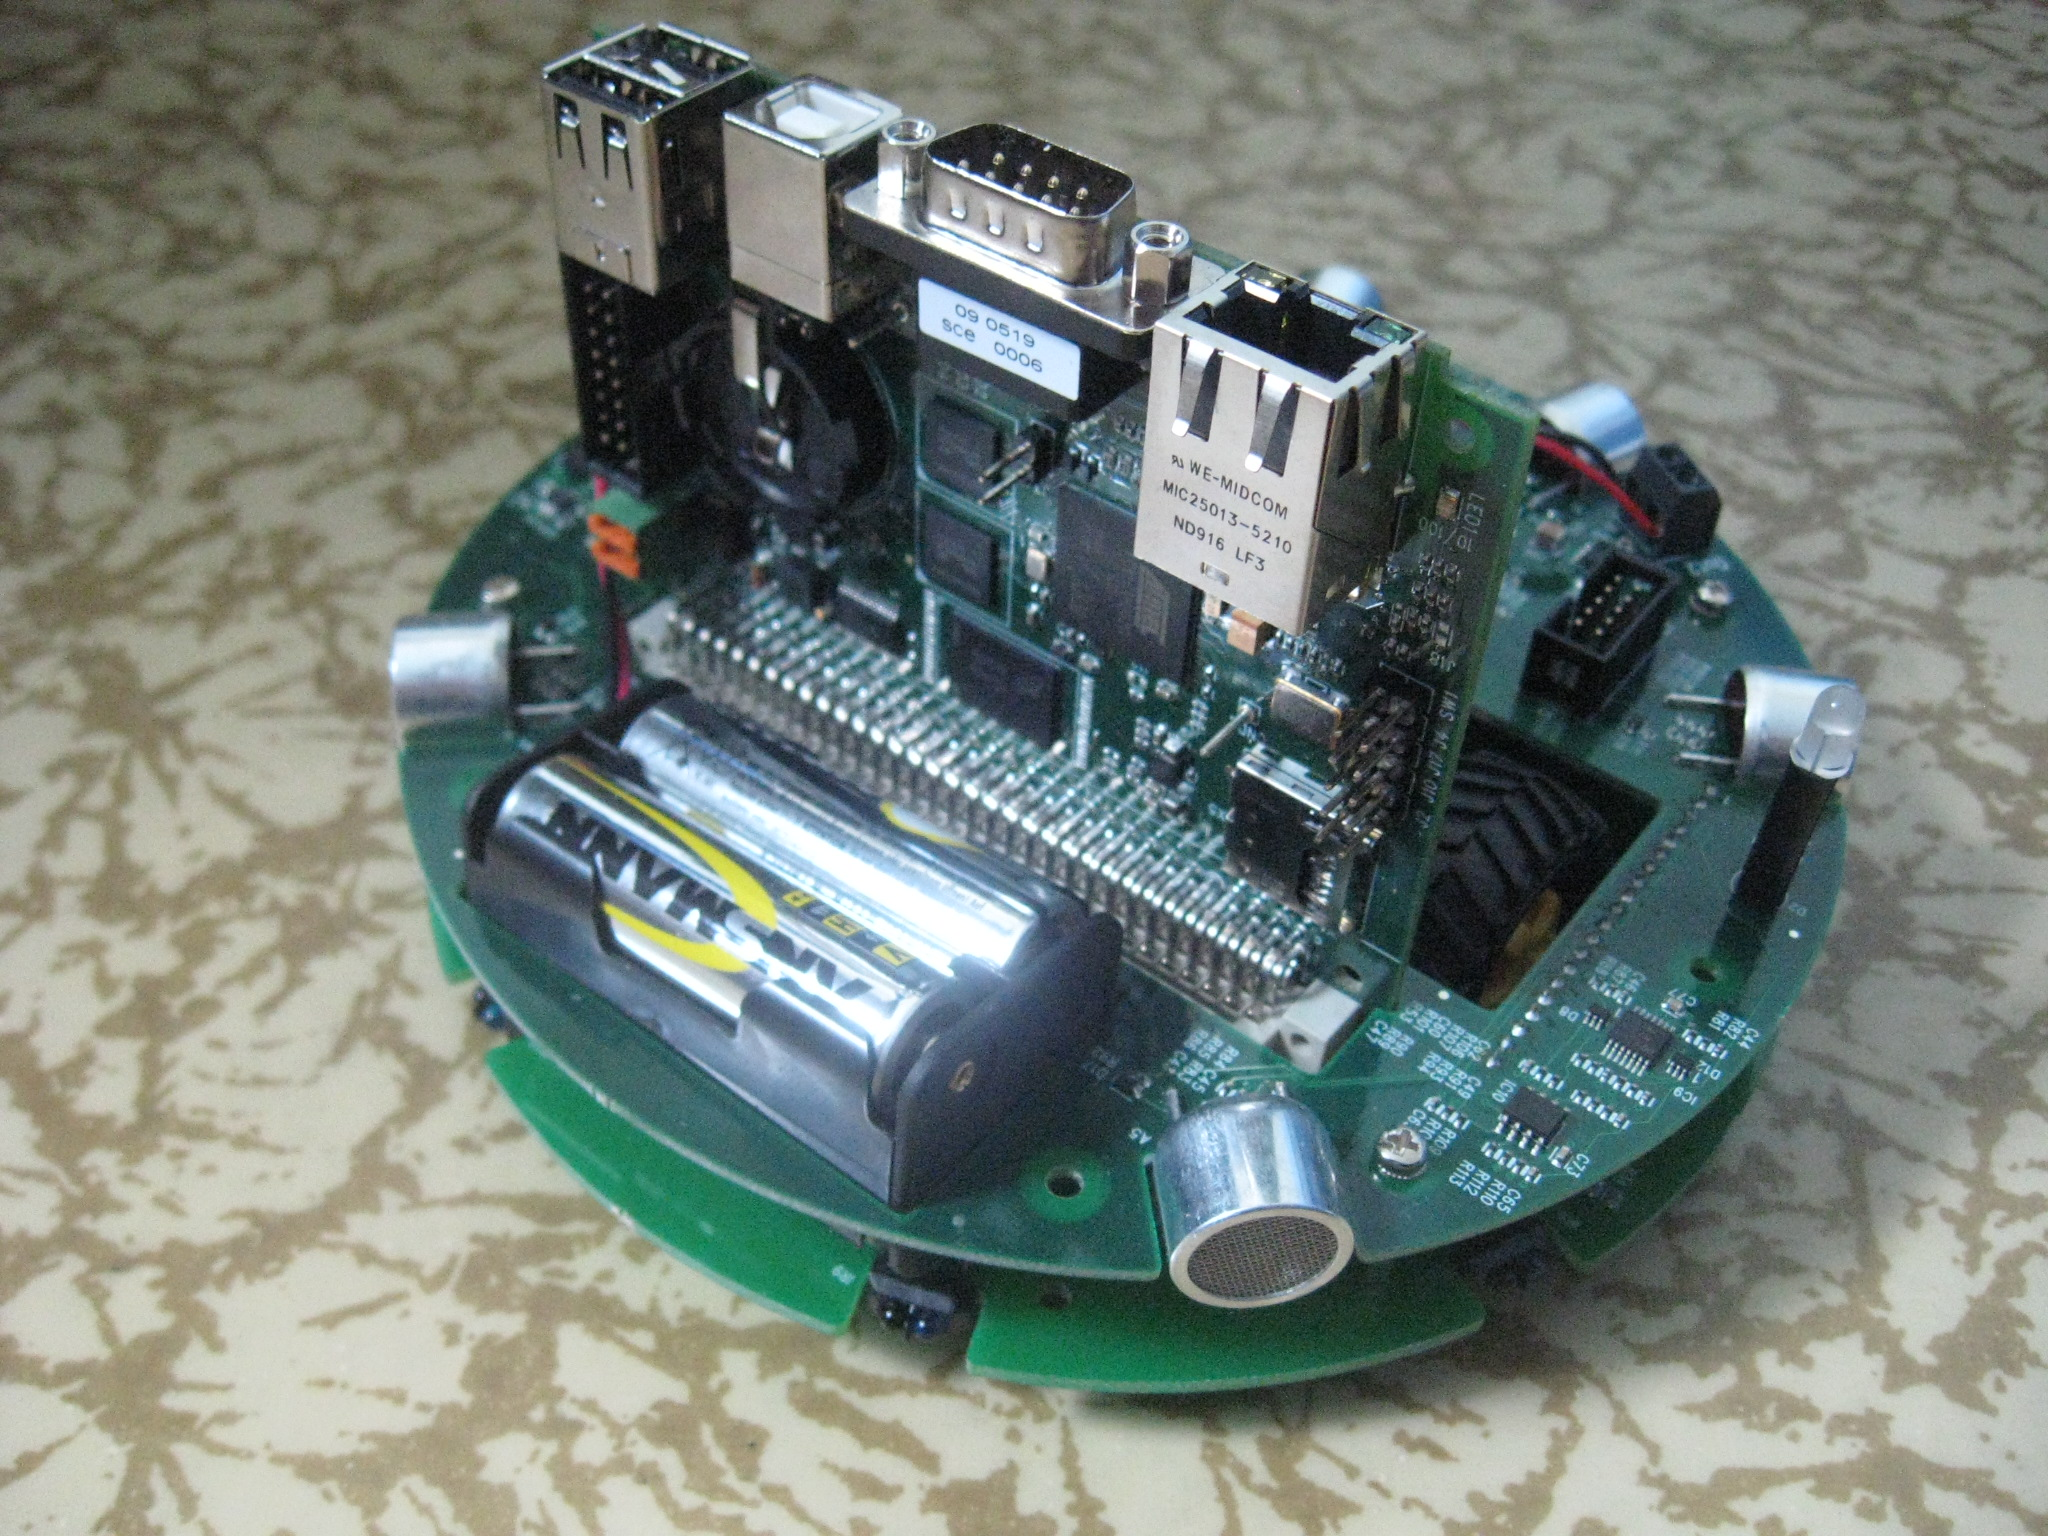
\includegraphics[width=\textwidth]{bilder/robo2.jpg}
				\caption{Schwarmelement von hinten}
			\end{figure}
		\end{column}
	\end{columns}
\end{frame}

\note{
	Vorstellen der Schwarmelemente, bevor die Architektur betrachtet wird
	
	Hier sind zwei in echter Gr\"o"sse.. (Zeigen/Rumgeben)
	f\"ur diejenigen, die diese noch nicht kennen
}

%----------------------------------------------------------------

\begin{frame}[label=Kamerasystem]
	\frametitle{System}\framesubtitle{Flexible Ortung von Schwarmelementen im Innenraum\\
		auf Basis kosteng\"unstiger Kameras}
	\begin{figure}
		\centering
		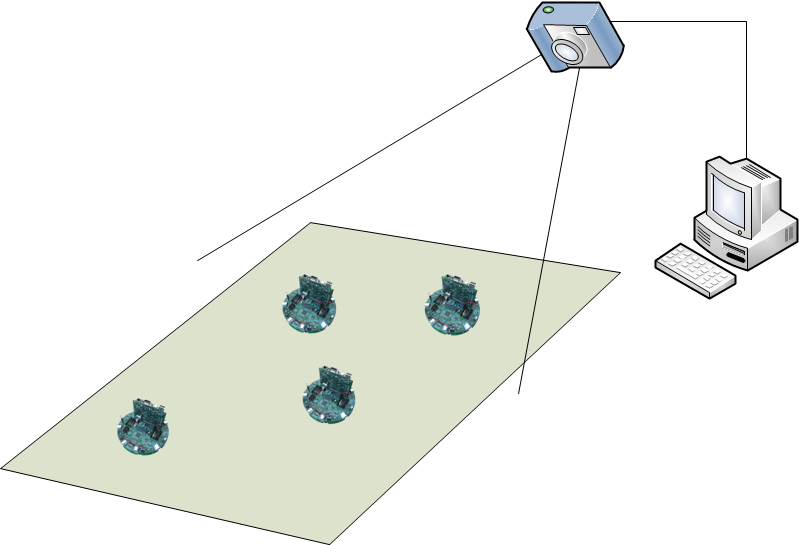
\includegraphics[height=60mm]{bilder/Kamerasystem.png}
		\caption{Architektur}
	\end{figure}
\end{frame}

\note{
	\begin{enumerate}
	  	\item Architektur: Schwarmelemete fahren auf dem Boden herum
	  	\item Kamera beobachtet diese, ohne sich selbst zu bewegen
	  	\item an einem Computer werden die von der kamera aufgenommenen daten verarbeitet
	\end{enumerate}
	\begin{enumerate}
	  	\item --- Analysieren des Titels der Bachelorarbeit.. ---
		\item Ortung: Bestimmung der Position des Schwarmelements
		\item Umgebung: Innenraum - begrenztes Feld (W\"ande / eigene Definitionen)
		\item Flexible Ortung: Winkel der Kamera flexibel oder mehrere Kameras verwenden oder beides 
		\item Was sind kosteng\"unstige Kameras ???
		\item Eigenes Ziel: das Programm flexibel gestalten
	\end{enumerate}
}

%----------------------------------------------------------------

\subsection[Kameras]{Kosteng\"unstige Kameras}

%----------------------------------------------------------------

\begin{frame}
	\frametitle{Kosteng\"unstige Kameras}\framesubtitle{Ideale Kamera (Lochkamera)}
	\begin{columns}
		\begin{column}<+->{0.5\textwidth}
			\centering
			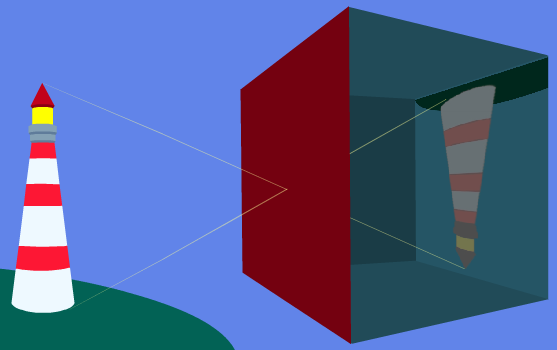
\includegraphics[width=1\textwidth]{bilder/lochkamera_scharf.PNG}\\
			scharf und dunkel \\lange Belichtungszeit
		\end{column}
		\begin{column}<+->{0.5\textwidth}
			\centering
			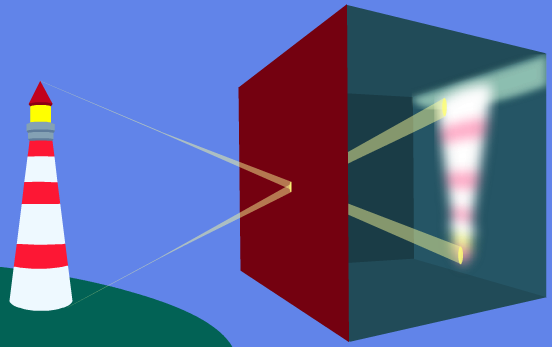
\includegraphics[width=1\textwidth]{bilder/lochkamera_unscharf.PNG}\\
			unscharf und hell \\kurze Belichtungszeit
		\end{column}
	\end{columns}
	\vskip28pt
	\footnotesize \color{gray}{Quelle: http://www.planet-schule.de/sf/multimedia-interaktive-\\
	\hskip30pt animationen-detail.php?projekt=lochkamera~(SWR/WDR~2011)}
\end{frame}

%----------------------------------------------------------------

\begin{frame}
	\frametitle{Kosteng\"unstige Kameras}\framesubtitle{Reale Kamera}
	\begin{block}<+->{Von der idealen zur realen Kamera}
		\begin{itemize}
		  \item Benutzen von Linsen zur B\"undelung des Lichts (Objektiv)\note[item]{Gewinnung von Sch\"arfe bei gleichbleibender Lochgr\"o"sse, Einstellung der Entfernung}
		  \item Einstellung der mechanischen Blende\note[item]{Regulierung der Lochgr\"o"sse zur Verk\"urzung der Belichtungszeit}
		\end{itemize}
	\end{block}
	
	\begin{block}<+->{Kosteng\"unstig}
		\begin{description}
		  \item[$\hookrightarrow$] Keine Entfernungseinstellung m\"oglich (Fixfokus-Objektiv)\note[item]{Fokus liegt im ``Unendlichen''}
		  \item[$\hookrightarrow$] Keine mechanische Blende vorhanden\note[item]{keine automatische Einstellung der Blende}
		  \item[$\Rightarrow$] ``Schnappschuss-Einstellung''\note[item]{immer gleiche Belichtungszeit}
		  \item[Bsp.:] \color{green!60!black}{Webcams}\note[item]{immer gleiche Belichtungszeit}
		\end{description}
	\end{block}
\end{frame}

%----------------------------------------------------------------

\begin{frame}
	\frametitle{Kosteng\"unstige Kameras}\framesubtitle{Verzeichnungen 1: radial-symmetrisch}
	\centering
	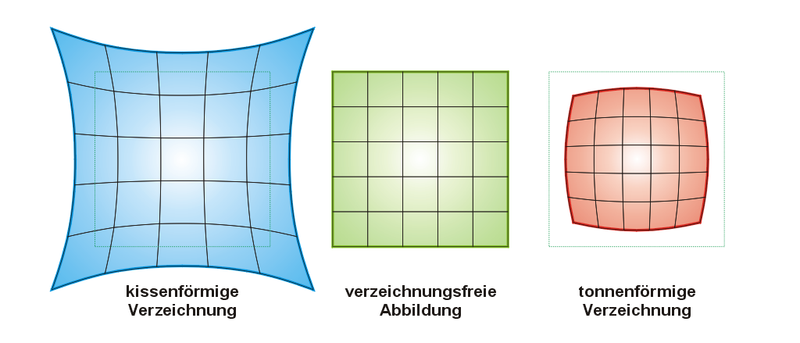
\includegraphics[width=1\textwidth]{bilder/Verzeichnung.png}\\
	\hskip110pt \footnotesize \color{gray}{(Author: Fantagu)}
\end{frame}

%----------------------------------------------------------------

\begin{frame}
	\frametitle{Kosteng\"unstige Kameras}\framesubtitle{Verzeichnungen 2: tangential-(a)symmetrisch}
	\centering
	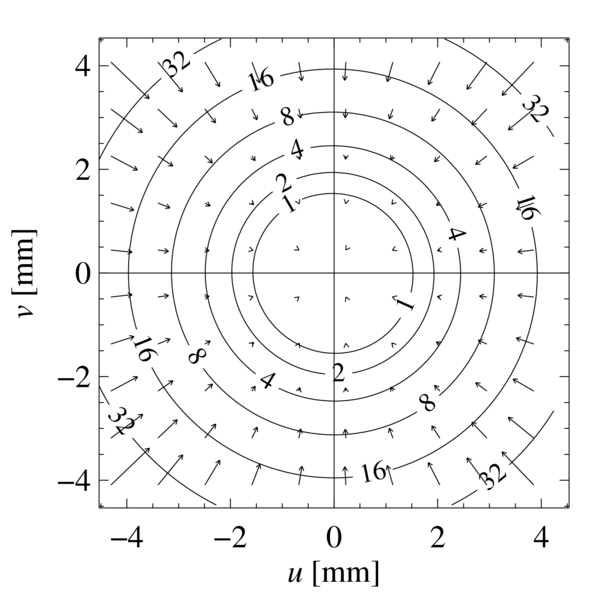
\includegraphics[width=0.65\textwidth]{bilder/Verzeichnung2.png}\\
	\hskip110pt \footnotesize \color{gray}{(Author: Georg Wiora)}
\end{frame}

%----------------------------------------------------------------

\begin{frame}[label=Kamerasystem2]
	\frametitle{Kosteng\"unstige Kameras}\framesubtitle{Koordinatensysteme}
	\begin{figure}
		\centering
		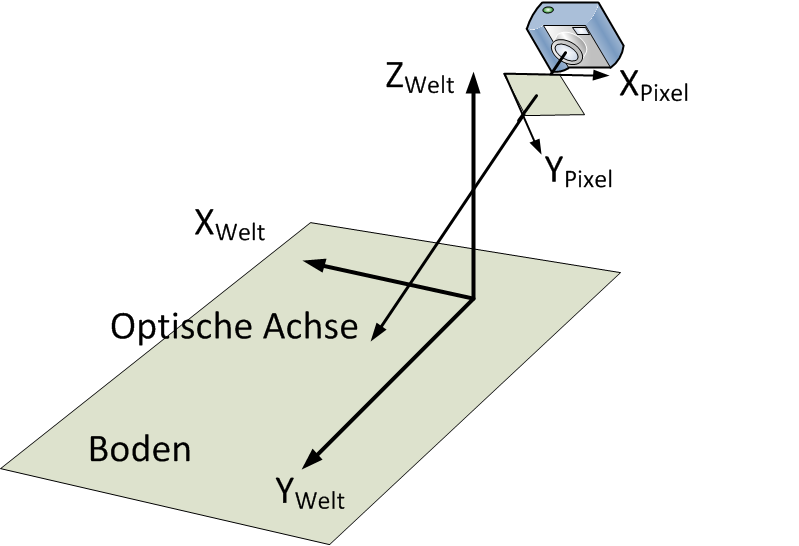
\includegraphics[height=60mm]{bilder/Kamerasystem2.png}
		\caption{Bild-, Kamera- und Weltkoordinatensystem im Vergleich;
		\"Au"sere~und~innere~Orientierung}
	\end{figure}
\end{frame}

%----------------------------------------------------------------

\againframe{Kamerasystem}

%----------------------------------------------------------------

\againframe{Kamerasystem2}

\note{Korrektur dieser Verzeichnungen:
	\begin{itemize}
	  \item Verfahren gruppiert nach Einbildkalibrierung und Mehrbildkalibrierung
	  \item Sch\"atzwerte vorhanden oder nicht?
	  \item Nahbereichsphotogammetrie
	  \item Kalibrierung: Bestimmung verschiedener Kamera- und Verzeichnungsparameter
	\end{itemize}
}

%----------------------------------------------------------------

\subsection[Ansatz]{Ansatz zur Probleml\"osung}

%----------------------------------------------------------------

\begin{frame}
	\frametitle{Ansatz zur Probleml\"osung}
	\begin{block}<+->{Vorgehen}
		\begin{enumerate}
		  \hilite<1> \item \textbf{Kalibrierung} der Kamera: Genauigkeitserh\"ohung
		  \hilite<2> \item \textbf{Positionsbestimmung} -- \\Umrechnung: Bild- $\Leftrightarrow$ Weltkoordinaten
		  \hilite<3> \item \textbf{Detektion} und Berechnung der Position der Schwarmelemente
		  \hilite<4> \item Aktualisierung dieser Position durch die \textbf{Verfolgung} des Schwarmelements
		\end{enumerate}
	\end{block}
\end{frame}

%================================================================
%================================================================

\section{Umsetzung}

%----------------------------------------------------------------

\begin{frame}\frametitle{Inhaltsverzeichnis}\framesubtitle{Kalibrierung}
\tableofcontents[currentsection, hideothersubsections]
\end{frame}

%================================================================

\subsection{Kalibrierung}

%----------------------------------------------------------------

\begin{frame}
	\frametitle{Kalibrierung}\framesubtitle{Vorlagen eines
	Kalibrierobjekts}
	\begin{columns}
		\begin{column}{0.45\textwidth}
			\centering
			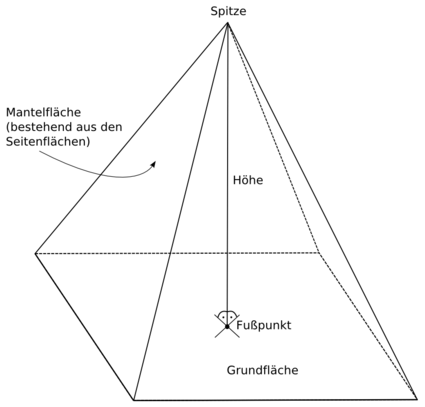
\includegraphics[width=1\textwidth]{bilder/Pyramide.png}\\
			3D-Kalibrierobjekt
		\end{column}
		\begin{column}{0.1\textwidth}
			\centering
			vs.
		\end{column}
		\begin{column}{0.45\textwidth}
			\centering
			
\includegraphics[width=1\textwidth]{bilder/schachbrett.png}\\
			2D-Kalibrierobjekt
		\end{column}
	\end{columns}
\end{frame}



%----------------------------------------------------------------

\begin{frame}
	\frametitle{Kalibrierung}\framesubtitle{Zwei
	bekannte Kalibrierverfahren}
	\begin{columns}
		\begin{column}{0.45\textwidth}
			\centering
			\begin{block}{DLT}
				\begin{enumerate}
				  \hilite<1> \item Punktkorrespondenzen
				  \hilite<2> \item verteilte Objektkoord.
				  \hilite<3> \item ein Bild ausreichend
				  \hilite<4> \item unbekannte Orientierung
				  \hilite<5> \item nicht-lineare Verzerrungen\\nicht korrigiert
				\end{enumerate}
			\end{block}
		\end{column}
		\begin{column}{0.1\textwidth}
			\centering
			vs.
		\end{column}
		\begin{column}{0.45\textwidth}
			\centering
			\begin{block}{Verfahren nach Zhang}
				\begin{enumerate}
				  \hilite<1> \item Punktkorrespondenzen
				  \hilite<2> \item planare Objektkoord.
				  \hilite<3> \item mehrere Bilder
				  \hilite<4> \item unbekannte Orientierung\textbf{en}
				  \hilite<5> \item nicht-lineare Verzerrungen\\korrigiert
				\end{enumerate}
			\end{block}
		\end{column}
	\end{columns}
\end{frame}

\note{
	Vorteile DLT:
	- nur ein Bild: innere und äußere Orientierung in einem Rutsch
	resultierende Nachteile:
	- $\Rightarrow$ jedesmal kalibieren -- innere orientierung muss so exakt wie möglich sein
		(gleichungen sind nicht nach innerer und äußerer getrennt) ???
	- $\Rightarrow$ 3D-Objekt muss exakt/genau sein
	- $\Rightarrow$ verteilte Objektkoordinaten müssen genau sein (manche Punkte nicht so genau bestimmbar)
	Vorteile Zhang: 
	- 2D-Objekt einfach herzustellen und zu transportieren
	(z.B. einfahc ausdrucken)
	- Kein Problem mehrere Bilder zu machen
	- Kalibrierung geschieht nur beim ersten Mal (und in regelmäßigen Abständen)
}

%----------------------------------------------------------------

\subsection[Position]{Bestimmen der Position}

%----------------------------------------------------------------

\begin{frame}
	\frametitle{Bestimmen der Position}\framesubtitle{Grundlagen}
	\begin{block}<+->{Vorgehen}
		\begin{enumerate}
		  \item TODO
		\end{enumerate}
	\end{block}
\end{frame}

%----------------------------------------------------------------

\begin{frame}
	\frametitle{Bestimmen der Position}\framesubtitle{Durchf\"uhrung}
	\begin{block}<+->{Vorgehen}
		\begin{enumerate}
		  \item TODO
		\end{enumerate}
	\end{block}
\end{frame}

%----------------------------------------------------------------

\begin{frame}
	\frametitle{Bestimmen der Position}\framesubtitle{Auswertung}
	\begin{block}<+->{Vorgehen}
		\begin{enumerate}
		  \item TODO
		\end{enumerate}
	\end{block}
\end{frame}

%----------------------------------------------------------------

\subsection[Detektion]{Detektieren der Schwarmelemente}

%----------------------------------------------------------------

\begin{frame}
	\frametitle{Detektieren der Schwarmelemente}\framesubtitle{Grundlagen}
	\begin{block}<+->{Vorgehen}
		\begin{enumerate}
		  \item TODO
		\end{enumerate}
	\end{block}
\end{frame}

%----------------------------------------------------------------

\begin{frame}
	\frametitle{Detektieren der Schwarmelemente}\framesubtitle{Durchf\"uhrung}
	\begin{block}<+->{Vorgehen}
		\begin{enumerate}
		  \item TODO
		\end{enumerate}
	\end{block}
\end{frame}

%----------------------------------------------------------------

\begin{frame}
	\frametitle{Detektieren der Schwarmelemente}\framesubtitle{Auswertung}
	\begin{block}<+->{Vorgehen}
		\begin{enumerate}
		  \item TODO
		\end{enumerate}
	\end{block}
\end{frame}

%----------------------------------------------------------------

\subsection[Verfolgung]{Verfolgen der Schwarmelementbewegung}

%----------------------------------------------------------------

\begin{frame}
	\frametitle{Verfolgen der Schwarmelementbewegung}\framesubtitle{Grundlagen}
	\begin{block}<+->{Vorgehen}
		\begin{enumerate}
		  \item TODO 
		\end{enumerate}
	\end{block}
\end{frame}

%----------------------------------------------------------------

\begin{frame}
	\frametitle{Verfolgen der Schwarmelementbewegung}\framesubtitle{Durchf\"uhrung}
	\begin{block}<+->{Vorgehen}
		\begin{enumerate}
		  \item TODO
		\end{enumerate}
	\end{block}
\end{frame}

%----------------------------------------------------------------

\begin{frame}
	\frametitle{Verfolgen der Schwarmelementbewegung}\framesubtitle{Auswertung}
	\begin{block}<+->{Vorgehen}
		\begin{enumerate}
		  \item TODO
		\end{enumerate}
	\end{block}
\end{frame}

%================================================================
%================================================================

\section[Implementation]{Implementierungsaspekte}

%----------------------------------------------------------------

\begin{frame}\frametitle{Inhaltsverzeichnis}
\tableofcontents[currentsection, hideothersubsections]
\end{frame}

%----------------------------------------------------------------

\subsection[Kalibrierung]{Kamerakalibrierung}

%----------------------------------------------------------------

\begin{frame}
	\frametitle{Kamerakalibrierung}\framesubtitle{Programm}
	\begin{block}<+->{Vorgehen}
		\begin{enumerate}
		  \item TODO
		\end{enumerate}
	\end{block}
\end{frame}

%----------------------------------------------------------------

\subsection[Flexible Ortung]{Flexible Ortung von Schwarmelementen}

%----------------------------------------------------------------

\begin{frame}
	\frametitle{Flexible Ortung von Schwarmelementen}\framesubtitle{Programm}
	\begin{block}<+->{Vorgehen}
		\begin{enumerate}
		  \item TODO
		\end{enumerate}
	\end{block}
\end{frame}

%================================================================
%================================================================

\section[Fazit]{Schlussbemerkungen}

%----------------------------------------------------------------

\begin{frame}\frametitle{Inhaltsverzeichnis}
\tableofcontents[currentsection, hideothersubsections]
\end{frame}

%================================================================

\subsection{Ausblick}

%----------------------------------------------------------------

\begin{frame}
	\frametitle{Ausblick}
	\begin{block}<+->{Vorgehen}
		\begin{enumerate}
		  \item TODO
		\end{enumerate}
	\end{block}
\end{frame}

%----------------------------------------------------------------

\subsection{Zusammenfassung}

%----------------------------------------------------------------

\begin{frame}
	\frametitle{Zusammenfassung}\framesubtitle{Flexible Ortung von Schwarmelementen im Innenraum auf Basis kosteng\"unstiger Kameras}
	\begin{block}<+->{Vorgehen}
		\begin{enumerate}
		  \item TODO
		\end{enumerate}
	\end{block}
\end{frame}

%----------------------------------------------------------------

\begin{frame}
	\frametitle{Zusammenfassung}\framesubtitle{Quellen \& Literatur}
%\begin{thebibliography}{9}
%\bibitem[Beamerpaket]{paket} \emph{Beamer Paket} \\ \text{http://www.taucher.net/photos/photo42/tauchfotos_Luzon__Palawan_Philippinen.html}
%\bibitem[Beamerdokumentation]{doku} \emph{User's Guide to the Beamer} 
%\bibitem[Dante]{dante} \emph{DANTE e.V.} \text{http://www.dante.de}   
%\end{thebibliography}
\end{frame}

%----------------------------------------------------------------

\begin{frame}
	\frametitle{Zusammenfassung}\framesubtitle{Flexible Ortung von Schwarmelementen im Innenraum auf Basis kosteng\"unstiger Kameras}
	\vskip50pt
	\hskip50pt \structure{Vielen Dank f\"ur Ihre Aufmerksamkeit!}
\end{frame}

%----------------------------------------------------------------

\subsection{Diskussion}

%----------------------------------------------------------------

\begin{frame}
	\frametitle{Diskussion}\framesubtitle{Flexible Ortung von Schwarmelementen im Innenraum auf Basis kosteng\"unstiger Kameras}
	\begin{block}{Vorgehen}
		\begin{enumerate}
		  \item TODO
		\end{enumerate}
	\end{block}
\end{frame}

%================================================================
%================================================================

\end{document}
